\documentclass{article}
%\usepackage[utf8]{inputenc}
\usepackage[utf8]{vietnam}
\usepackage{amsmath,amsxtra,amssymb,latexsym, amscd,amsthm}
\usepackage{mathtools}
\usepackage{graphicx}
\usepackage{wrapfig}
\usepackage{blindtext}



\newcommand{\norm}[1]{\left\lVert#1\right\rVert}


\title{$p\,$-norm of matrices}
\author{phunc20}
\date{\today}


\begin{document}
\maketitle
\section{Động cơ}
%Tại sao người ta lại nghĩ đến định nghĩa $\Vert A \Vert := \sup_{\bold{x} \ne \bold{0}} \frac{A\bold{x}}{\Vert \bold{x} \Vert}$
%Tại sao người ta lại nghĩ đến định nghĩa $\Vert A \Vert \mathrel{\mathop:}= \sup_{\bold{x} \ne \bold{0}} \frac{A\bold{x}}{\Vert \bold{x} \Vert}$
%Tại sao người ta lại nghĩ đến định nghĩa $\Vert A \Vert \coloneqq \sup_{\bold{x} \ne \bold{0}} \frac{A\bold{x}}{\Vert \bold{x} \Vert}$
Tại sao người ta lại nghĩ đến định nghĩa norm của một ma trận $A \in M_{m,n}(\mathbb{C})$
$$\norm{A} \,\,\coloneqq\!\! \sup_{\mathbf{x} \,\in\, {\mathbb{C} \setminus \{\mathbf{0}\}}} \frac{\norm{A\mathbf{x}}}{\norm{\mathbf{x}}}\;$$
như thế này?


\begin{wrapfigure}{h}{0.5\textwidth}
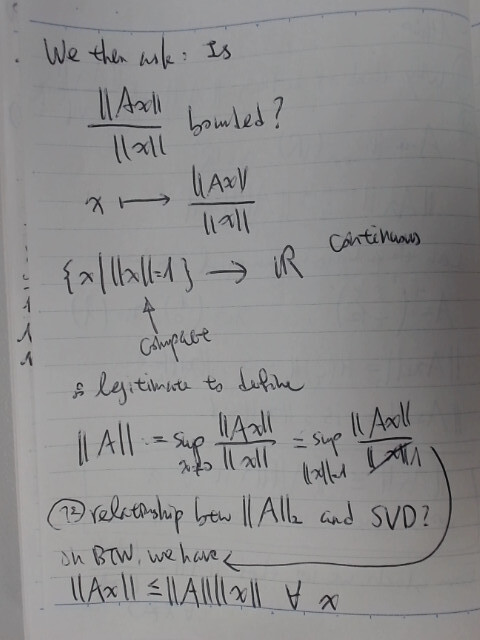
\includegraphics[width=0.4\textwidth]{02-moti_cont.jpg}
\end{wrapfigure}
\blindtext

\begin{wrapfigure}{p}{0.5\textwidth}
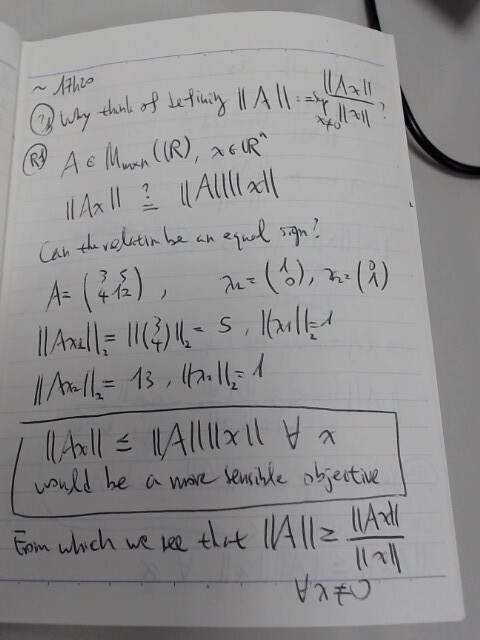
\includegraphics[width=0.4\textwidth]{01-motivation.jpg}
%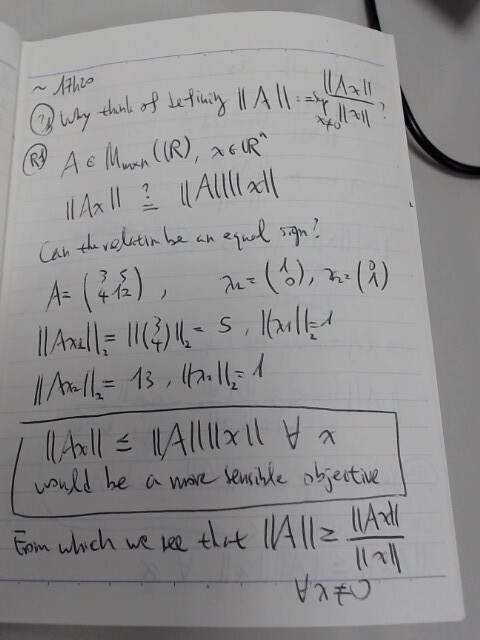
\includegraphics[width=2.5cm]{01-motivation.jpg}
%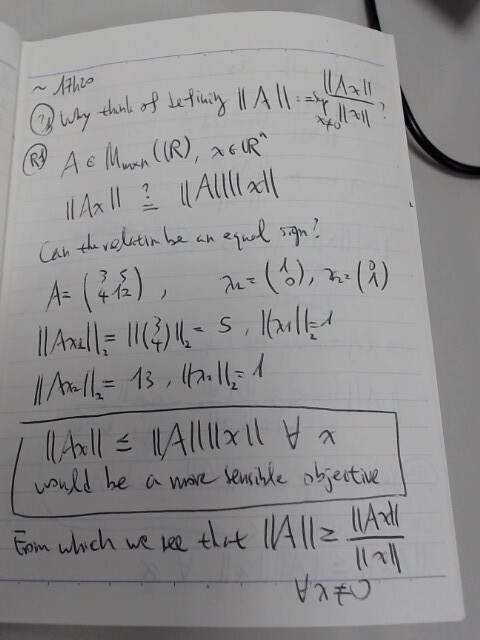
\includegraphics{01-motivation.jpg}
\end{wrapfigure}

\blindtext

%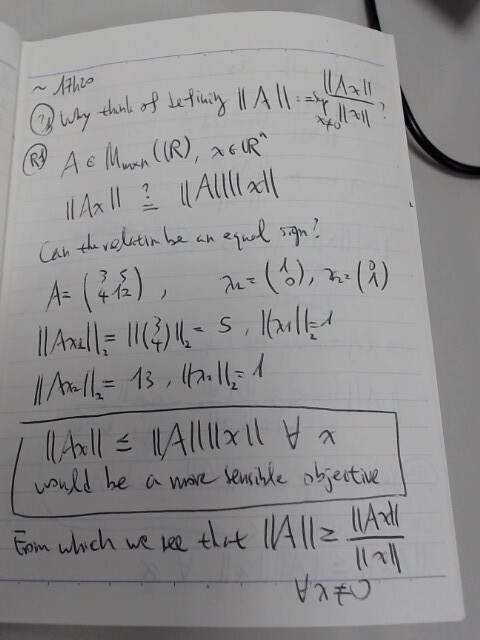
\includegraphics[width=0.7\textwidth]{01-motivation.jpg}
%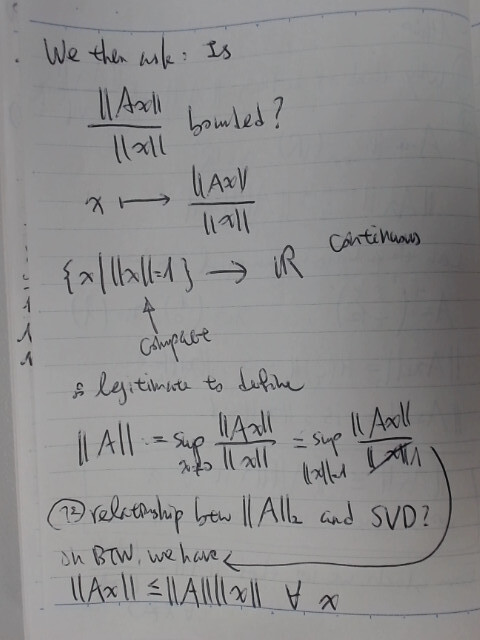
\includegraphics[width=0.7\textwidth]{02-moti_cont.jpg}
%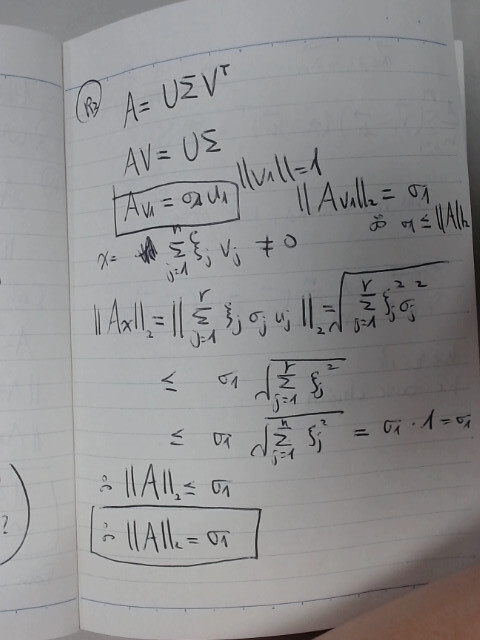
\includegraphics[width=0.7\textwidth]{03-2norm_and_singular_value.jpg}
%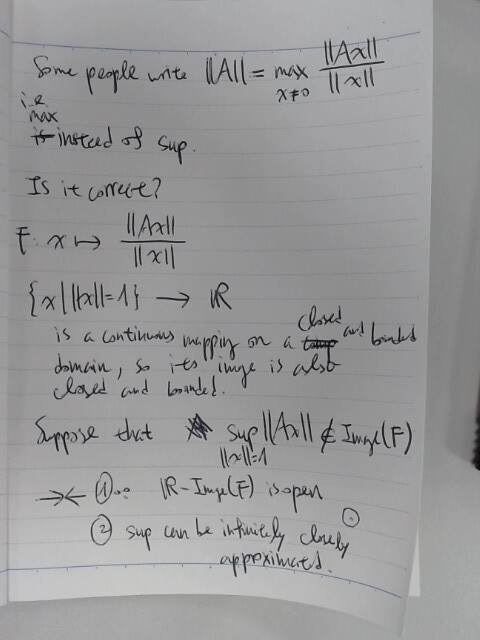
\includegraphics[width=0.7\textwidth]{04-max_instead.jpg}










\end{document}





%   01-motivation.jpg
%   02-moti_cont.jpg
%   03-2norm_and_singular_value.jpg
%   04-max_instead.jpg
%   covariance.jpg
%   decompression.jpg
%   motivation.tex
%   vietnamese.tex

